\documentclass[../main.tex]{subfiles}
\begin{document}
\chapter{Winds}\label{chapter3}
We set out to find continuous and monotonic solutions to the equations of structure \eqref{eq:dvdr}-\eqref{eq:dTdr} for a neutron star of mass $M=1.4\Msun$ and radius $R=12$ km. In these winds, the velocity $u$ should be small near the star's surface and accelerate outward against gravity, representing a progressive transfer of energy from gas enthalpy and radiation into kinetic energy.  Each solution to the equations is characterized by a unique set of two free parameters, the mass and energy loss rates $\Mdot$ and $\Edot$. 

Not every solution will be physically acceptable as a neutron star wind. Thus, boundary/initial conditions will have to be enforced. One will come from attaching the wind base to the surface of the star, another from the thermal definition of the photosphere. A third condition will appear from the requirement of a continuously accelerating solution, and follow naturally from a topological feature of the equations of structure. We begin this chapter by explaining this third condition in \S\ref{sec:critical_point}, then describe our numerical method along with the two other boundary conditions in \S\ref{sec:wind_numerical_method}. We then explain the root-finding method which leads to the final wind models in \S\ref{section:wind_rootfinding}, which we show and analyze in \S\ref{sec:wind_results}. Lastly, we discuss how our models relate to observations in terms of photospheric radii and spectral shifts in \S\ref{sec:wind_photospheres_spectralshifts}.

\section{The critical point}\label{sec:critical_point}
In the winds, as the velocity monotonically increases outward to infinity, the sound speed decreases with the square root of the temperature (see Eq.~\ref{eq:cs}). This means that the velocity will necessarily go from being subsonic to supersonic at some point. This point is the \textit{critical point}, located at $r=r_c$.  

The critical point, sometimes also called sonic point, has been a universal feature of stellar wind modeling since the first solar wind paper by \citet{Parker1958}. It is notable because it always appears as a singularity in the velocity gradient equation, no matter the choice of equation of state. In our case, for Eq.~\eqref{eq:dvdr}, the singularity occurs at the critical velocity $u=u_c\equiv \sqrt{B/A}$, with the determinant going to zero. Note that this is very close to the sound speed but not exactly it ($A\gtrsim 1$ because of GR corrections). In order for the velocity to smoothly pass through $r_c$, its derivative must be finite. This can only be possible if the numerator of Eq.~\eqref{eq:dvdr} is also exactly zero at the critical point, giving the constraint
\begin{equation}\label{eq:regularity_constraint}
    \left[\frac{GM}{r\zeta^2}\left(A-\frac{B}{c^2}\right)-2B-C\right]_{r=r_c,u=u_c}=0 \,.
\end{equation}

There will be numerical divergences in the vicinity of the critical point because both the numerator and denominator of $du/dr$ are close to zero and change sign exactly at $r_c$. Considering GR, this is even more of a problem because the velocity gradient also appears in the temperature gradient equation \eqref{eq:dTdr}. There have been several proposed methods for dealing with these instabilities. For example, \citet{Paczynski1986b} approximated $d\ln u/d\ln r\approx 1$ and $d\ln T/d\ln r\approx -1$ near $r_c$, and used these values to integrate away from the critical point until $du/dr$ became stable. \citet{Zytkow1972,Kato1983a} and \citet{Quinn1985} used analytical expansion formulas for $du/dr$ that would become very involved in the GR case. \citet{Joss1987} introduced a novel change of variables which immediately cancels the singular denominator, which is arguably the simplest and most elegant solution to the singularity problem. We introduce here a GR analog to the \citet{Joss1987}'s $\Phi$ variable,
\begin{equation}
    \label{eq:phi}
    \Phi=A^{1/2}\mach+\frac{1}{A^{1/2}\mach}\,,
\end{equation}
where $\mach=u/B^{1/2}$ is the usual mach number. $\Phi$ has a value of exactly 2 at $r=r_c$.  Since the non-degenerate parameters $A$,$B$,$C$ are functions of temperature only, the gradient takes the simple form
\begin{equation}
    \frac{d\Phi}{dr}=\frac{(A\mach^2-1)(3B-2Ac^2)}{4\mach A^{3/2}c^2r}
    \frac{d\ln T}{d\ln r}
    -\frac{B-Av^2}{vr\sqrt{AB}}\frac{d\ln u}{d\ln r}\,.
    \label{eq:dphidr}
\end{equation}
By substituting in equation \eqref{eq:dvdr} into the second term, we see that the denominator at the critical point cancels, and so we may use this expression to smoothly integrate around and through $r_\text{c}$.  As for the temperature gradient Eq.~\eqref{eq:dTdr}, the last term containing $du/dr$ (and therefore also the singularity) is small and may be ignored, as it will be shown that $u\sim 0.01c$ at most in the winds.

\section{Numerical integration and boundary conditions}\label{sec:wind_numerical_method}
To calculate wind solutions, we use an approach similar to \citet{Paczynski1986b} in that we start at the critical point and integrate outward to the photosphere and inward to the star's surface, checking if the boundary conditions are met at both ends and changing the free parameters until they are. Table \ref{tab:wind_locations} summarizes the conditions that are applied at the three locations, which we will explain in detail in this section. We apply the same procedure for every mass-loss rate $\Mdot$ in order to have a single wind model for each value.  All integrations are done using fully implicit ODE solvers provided by the \textit{SciPy} numerical package \citep{SciPy}. 

The critical point is first found based on a trial value for its temperature $T_c$ by finding the unique root to Eq.~\eqref{eq:regularity_constraint}. Not all values of $r_c$ are acceptable. For instance, if $T_c$ is too high, the critical point can be located at $r<R$, below the surface of the star, such that the wind would start off supersonic at the base - we do not accept solutions of this kind. 

We then integrate equations \eqref{eq:dTdr} and \eqref{eq:dphidr} for $T$ and $\Phi$, with initial values of $T_c$ and 2, outward until reaching a \textit{photosphere} at $r=r\ph$. We define the photosphere as the location where the \textit{optical depth parameter}
\begin{equation}\label{eq:taustar}
    \tau^*\equiv \rho\kappa r
\end{equation}
reaches a value of 3. This is only an approximation of the photosphere. It must be made because our treatment of radiative transfer is done under a pure optically thick approximation. But this use of $\tau^*$ as a proxy for the true optical depth can and has been justified, e.g. by \citet{Quinn1985}\footnote{See also \citet[Chapter~7.6]{Mihalas1978} for a more extensive discussion on spherically symmetric grey atmospheres.}. If our equations did allow integration past the photosphere and into the optically thick regions to any distance, we could calculate this true optical depth
\begin{equation}\label{eq:trueopticaldepth}
    \tau(r)=\int_r^\infty \rho(r')\kappa(r') \frac{dr'}{\zeta(r')}
\end{equation}
At large distances, $\kappa\approx \kappa_0$, $\zeta\approx 1$, and $u$ is nearly constant such that $\rho$ can be approximated as a power law
\begin{equation}
    \rho = \Mdot/(4\pi r^2 u\Psi) \approx  Cr^{-n}\,,
\end{equation}
with $n\gtrsim 2$. Then, at the photosphere we have
\begin{equation}\label{eq:tau_taustar_approx}
    \tau(r\ph)\approx\kappa_0C\int_{r\ph}^\infty \frac{dr'}{(r')^n}=\frac{\kappa_0 Cr\ph^{-(n-1)}}{n-1}=\frac{\tau^*(r\ph)}{n-1}\,,
\end{equation}
showing that the use of $\tau^*$ close to the photosphere is appropriate for these winds.  

Another condition for the photosphere is that the flux escaping it locally should reflect what is observed spectrally at infinity. For a thermally emitting region with effective temperature $T_\text{eff}$, the bolometric flux is $F_\text{bol}=\sigma T_\text{eff}^4$. Our photosphere should therefore also have the thermal condition $T\ph\equiv T(r\ph)=T_\text{eff}$. Combining both definitions leads to our outer boundary condition:
\begin{equation}\label{eq:wind_outerBC}
    L\ph=4\pi r\ph^2\sigma T\ph^4 \quad, \qquad r\ph=r(\tau^*=3)\,.
\end{equation}
This condition will not be satisfied in general, as we are simply ``shooting'' from the critical point, rather than enforcing it. When reaching $r\ph$, we register the \textit{outer boundary error} as $L\ph-4\pi r\ph^2\sigma T\ph^4$ for the root-finding procedure. Note that $\tau^*=3$ is used because \citet{Quinn1985} (Newtonian wind models that also treat optically thin regions) showed that $T=T_\text{eff}$ was always satisfied for $3<\tau^*<5$. Then, \citet{Paczynski1986b} showed that either value (3 or 5) led to similar results in their GR wind models. One can also see from Eq.~\eqref{eq:tau_taustar_approx} that $\tau
^*=3$ corresponds to $\tau$ of order unity, which is indeed what we usually expect for the photosphere of stellar atmospheres. Further, we found that it was not generally possible to reach smaller values of $\tau^*$ without diverging, which seems to be a limitation of the optically thick approximation. 

Then, we go back to the critical point, this time to integrate inwards. We do this in two parts. Firstly, we once again integrate $T$ and $\Phi$ but only until we reach $r=0.95 r_c$. The point of this is simply to step off of the critical point, using $\Phi$ to avoid any numerical problems. But then, we want to consider degenerate electron corrections to calculate the inner part of the wind, which $\Phi$ is not set up to do. So, we then switch to integrating $r$ and $T$ with $\rho$ as the independent variable, all the way down to the surface of the star, constructing equations for $dr/d\rho$ and  $dT/d\rho$ from Eq.~\eqref{eq:drhodr} and \eqref{eq:dTdr}. We use $\rho$ as the independent variable instead of $r$ at this stage because the inner part of the wind, near the surface, is in hydrostatic equilibrium and is geometrically thin. Integrating with $r$, a variable which changes very little while the others change by many orders of magnitude, would be less stable numerically. We stop the integration once we reach the base of the wind $r_b$, which we define as the location where the column depth $y$ reaches a value of $10
^8$ g cm$^{-2}$. The column depth,
\begin{equation}\label{eq:columndepth}
    y(r)\equiv \int_r^\infty \rho \frac{dr'}{\zeta(r')}\,,
\end{equation}
is a mass coordinate which is given by the integrated density above a particular point $r$, factoring in length contraction for the given metric. 

Having performed time-dependent cooling calculations of the burning layers in Type I X-ray bursts using the \textit{burstcool} code \citep{Cumming2004,Cumming2006}, we were able to identify this particular value of $10^8$ g cm$^{-2}$ for the column depth as a sensible and consistent location for the beginning of the outflows, or base of the wind. It is small enough that the pure helium assumption remains valid. At higher depths, we would expect a significant fraction of heavy elements as products of nuclear burning. But it is also large enough that the gas should not be in a radiation pressure dominated regime at the base. We will re-visit the validity of this statement when analyzing the results further.  

In hydrostatic equilibrium, the total pressure must compensate the gravitational pressure of all of the material above, which can be compactly written as
\begin{equation}
    P=gy\,,
\end{equation}
where
\begin{equation}\label{eq:g}
    g=\frac{GM}{R^2\zeta(R)}=\frac{GM}{R^2}\left(1-\frac{r_s}{R}\right)^{-1/2}
\end{equation}
is the effective surface gravity of the star. This allows us to calculate the column depth from the pressure. Our inner boundary condition is simply to require that the wind base be located at the surface of the star, that is
\begin{equation}\label{eq:wind_innerBC}
    r_b\equiv r(P/g=10^8) = R \,.
\end{equation}

The point of this boundary condition is mainly to fix the wind to the surface to properly compare different solutions, and to restrict the free parameters in order to have a single wind solution per value of $\Mdot$. It is not too different from the inner boundary condition of \citet{Paczynski1986b}, who required a fixed temperature of $10^{9.7}$ K at the surface. Once again, this boundary condition will not be satisfied in general, so we record the \textit{inner boundary error} as $r_b-R$.

\begin{table}[h]
    \centering
    \caption{Locations and conditions in the wind model}
    % \vspace*{3mm}
    \begin{tabular}{c|c|c}
        $r$ & Name & Condition   \\\hline
        $r_b$ & Wind base radius & Matching to stellar radius (Eq.~\ref{eq:wind_innerBC})\\
        $r_c$ & Critical radius & Regularity constraint (Eq.~\ref{eq:regularity_constraint}) \\
        $r\ph$ & Photospheric radius & Thermal constraint (Eq.~\ref{eq:wind_outerBC})
    \end{tabular}
    \label{tab:wind_locations}
\end{table}

\section{Root-finding}\label{section:wind_rootfinding}
An exact wind solution, respecting the inner and outer boundary conditions, is found for each value of $\dot{M}$ by performing a Newton-Raphson root-finding algorithm on the ($\dot{E}$, $T_c$) parameter space. Figure \ref{fig:errorspace_18_5} shows this parameter space for $\log\dot{M}=18.5$. The white lines indicate the minima of the errors on the boundary conditions. For this value of $\log\dot{M}$, we can see that the root, located at the intersection of the two lines, is $\dot{E}\approx 9.11\Ledd$, $T_c\approx 10
^{7.2}$ K.  

\begin{figure}[htb!]
    \centering
    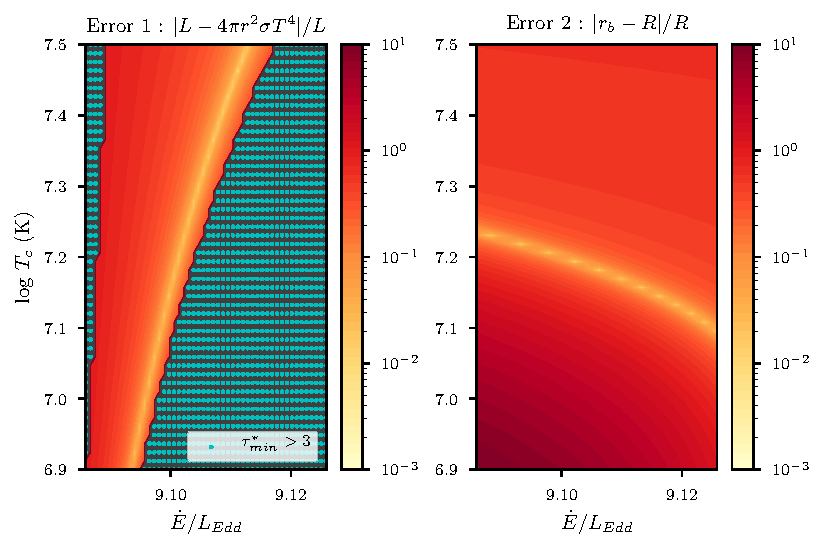
\includegraphics[width=\textwidth]{figures/errorspace_18_5.pdf}
    \caption[B.C. errors on the $\log\dot{M}=18.5$ wind parameter space]{Boundary condition errors on the ($\dot{E},T_c$) parameter space for $\log\dot{M}=18.5$. \textit{Left}: Outer boundary error of Eq.~\eqref{eq:wind_outerBC} (``ph'' subscripts omitted in the subplot title). \textit{Right}: Inner boundary error of Eq.~\eqref{eq:wind_innerBC}. The absolute value of the normalized errors are shown for clarity. Blue points represent free parameter values for which integration to the photosphere was not possible due to $\tau^*$ rising before reaching a value of 3.}
    \label{fig:errorspace_18_5}
\end{figure}

In order to automatically find the roots at every $\dot{M}$ without having to fully calculate the errors on the parameter space as in Fig.~\ref{fig:errorspace_18_5}, we implemented a custom Newton-Raphson searching algorithm, which essentially does a two-dimensional gradient descent towards the global minimum, with back-tracking and numerical error catching when approaching regions of divergence, such as the blue dotted region in Fig.~\ref{fig:errorspace_18_5} (see figure caption for explanation). We encountered other types of divergence at lower values of $\dot{M}$, which we show along with other parameter spaces in Appendix \ref{appendix_errospaces}. 

The result of the root-finding method are shown in figure \ref{fig:wind_roots}. One striking is feature of the root curve is the turnover in $T_c$ at low $\Mdot$. Indeed, instead of the critical point temperature continuing to increase as $\Mdot$ decreases, it starts to decrease at $\Mdot\lesssim 10^{18}$ g/s. This causes the critical point to become further from the surface and closer to the photosphere as $\Mdot$ decreases. At even lower values of $\Mdot$, the critical point would eventually go past the photosphere, and our method would not allow the calculation of these models. A similar behavior of the critical point was obtained by \citet{Paczynski1986b}. 

In the left panel of Fig.~\ref{fig:wind_roots}, we represented the $\Edot$ free parameter as $\Edot-\Mdot c^2$ to look at the energy loss rate without the rest mass contribution. What we see is that the remaining contributions to the energy loss rates are roughly constant and just above $\Ledd$. To explain this, we can take the energy conservation equation \eqref{eq:Edot} and evaluate it at infinity:
\begin{align}\label{eq:Edot_at_infty_approx}
    &\Edot=\Mdot\Psi_\infty \left(\frac{\omega_{g,\infty}+4/3U_{R,\infty}}{\rho_\infty}\right)+\left(\frac{1+u_\infty^2/c^2}{1-u_\infty^2/c^2}\right)L^\infty\nonumber\\
    &\Edot-\Mdot c^2\approx \Mdot c^2(\gamma_\infty-1) + \Mdot\gamma_\infty\left(\frac{kT_\infty}{\mu m_H}+\frac{4aT_\infty^4}{3\rho_\infty}\right)\nonumber\\
    &\qquad\qquad\qquad+\gamma_\infty^2(1+u_\infty^2/c^2)L^\infty\,,
\end{align}
where $\gamma_\infty$ is the Lorentz factor for $u_\infty$. The second expression shows that $u_\infty$ essentially dictates the small variance of the $\Edot-\Mdot c^2$ values in Fig.\ref{fig:wind_roots}. Indeed, the second term can be neglected since, naturally, $T_\infty\rightarrow0$. In the third term, the comoving luminosity just happens to be the constant $\Ledd$, as we will see and explain in the next section. All that is left is terms of $u_\infty$. \citet{Paczynski1986b} give the following estimate for the velocity at infinity,
%In the second expression, the main contribution is the third term. At infinity, the comoving luminosity just happens to be $\sim\Ledd$, as we will see and explain in the next section. The second term can be neglected since naturally $T_\infty\rightarrow0$. The first term is small but does contribute. Essentially, the specifics of the velocity profile, and in particular the value of $u_\infty$ explain the small variance of $\Edot-\Mdot c^2$ seen in the left panel of Fig.~\ref{fig:wind_roots}. \citet{Paczynski1986b} give the following estimate for the velocity at infinity,
\begin{equation}\label{eq:vinf}
    u_\infty^2 \approx u\ph^2 - \frac{GM}{r\ph}\left(1-\frac{L\ph}{\Lcr}\right)\, ,
\end{equation}
saying that past the photosphere, kinetic energy will be lost in order to escape the effective gravitational pull of the star. Fig.~\ref{fig:wind_vinf} shows $u_\infty$ as a function of $\Mdot$ according to Eq.~\eqref{eq:vinf}. We see that it peaks in between $\Mdot=10^{18}$ and $10^{18.5}$ g s$^{-1}$, which is consistent with our Eq.~\eqref{eq:Edot_at_infty_approx} and Fig.~\ref{fig:wind_roots}. 

Lastly, the bottom right panel of Fig.~\ref{fig:wind_roots} shows that the base luminosity, redshifted to infinity, levels off at high $\Mdot$. This is the first indication that the high mass-loss rate models are not valid. Indeed, it is a strange and likely non-physical conclusion that by increasing the base luminosity by only a few percent, the mass-loss rate could more than triple. A possible explanation is that for these models, the wind base is too shallow at $y=10^8$ g cm$^{-2}$, and should instead be deeper into the burning layer where the luminosity could keep increasing and follow the natural progression of the $L_b^\infty$ curve in Fig.~\ref{fig:wind_roots}. We will analyze in more detail in the next section if these high $\Mdot$ winds are in the same regime near the base as the others.


\begin{figure}[htb!]
    \centering
    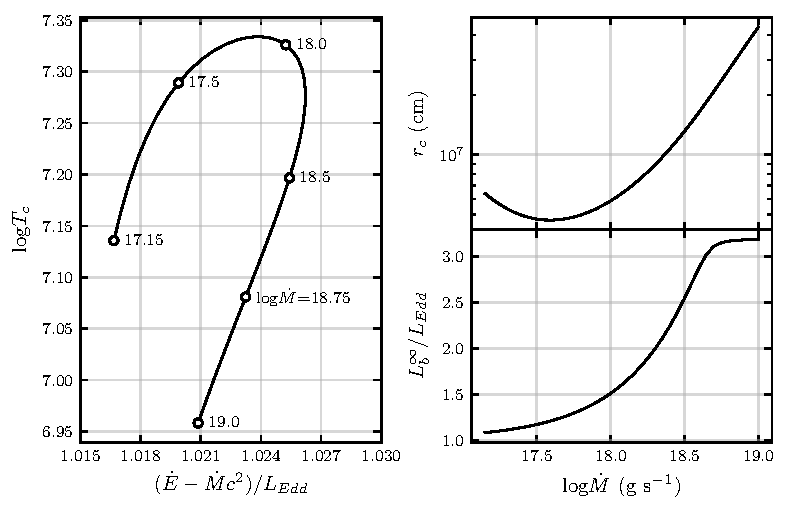
\includegraphics[width=\textwidth]{figures/wind_roots.pdf}
    \caption[Roots of wind models]{Roots of the wind models. \textit{Left}: ($\Edot,T_c$) parameter space, with sample values of $\log\Mdot$ labelled along the root curve. \textit{Right}: Critical point radius and base luminosity seen at infinity as a function of $\log\Mdot$, with each dot representing one of the computed models.}
    \label{fig:wind_roots}
\end{figure}

\begin{figure}[htb!]
    \centering
    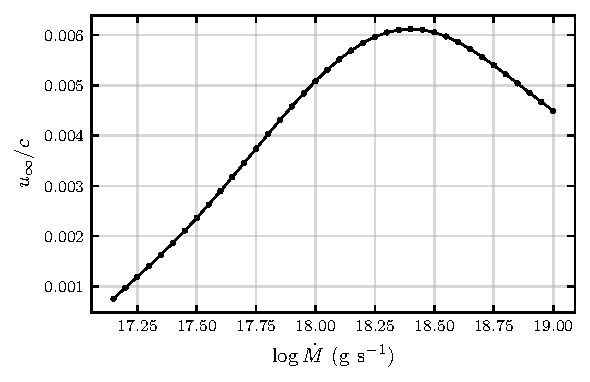
\includegraphics{figures/wind_vinf.pdf}
    \caption[Velocity at infinity of wind models]{Velocity at infinity according to Eq.~\eqref{eq:vinf}.}
    \label{fig:wind_vinf}
\end{figure}


% \section{Results}\label{sec:wind_results}
\section{Dependence of the wind models on $\Mdot$}\label{sec:wind_results}

We calculated wind models with the method described in Section \ref{sec:wind_numerical_method}, using the roots found in Section \ref{section:wind_rootfinding}. Figure \ref{fig:wind_profiles} shows the radial profiles of the winds for eight $\Mdot$ values. In all models, the wind base $r_b=12$ km has a high temperature and density. The inner part of the wind has very small velocities in all models. Since the sound speed scales with temperature, the mach numbers at the base are all smaller than $10^{-6}$, which justifies our assumption of hydrostatic equilibrium for the inner part of the wind.   

Near the surface, the flux seen at infinity is strongly super-Eddington, but rapidly decreases as the velocity increases, until it becomes only slightly higher than the Eddington luminosity (dotted line in the luminosity panel). This demonstrates how the super-Eddington flux is transfered to the gas in order to accelerate it. At large distances from the star, the gas stops being accelerated as it decouples from the radiation, and the luminosity remains just slightly super-Eddington simply through conservation of energy. This is also consistent with the fact that PRE bursts usually have a constant luminosity during the expansion phase.  

\begin{figure}[htb!]
    \centering
    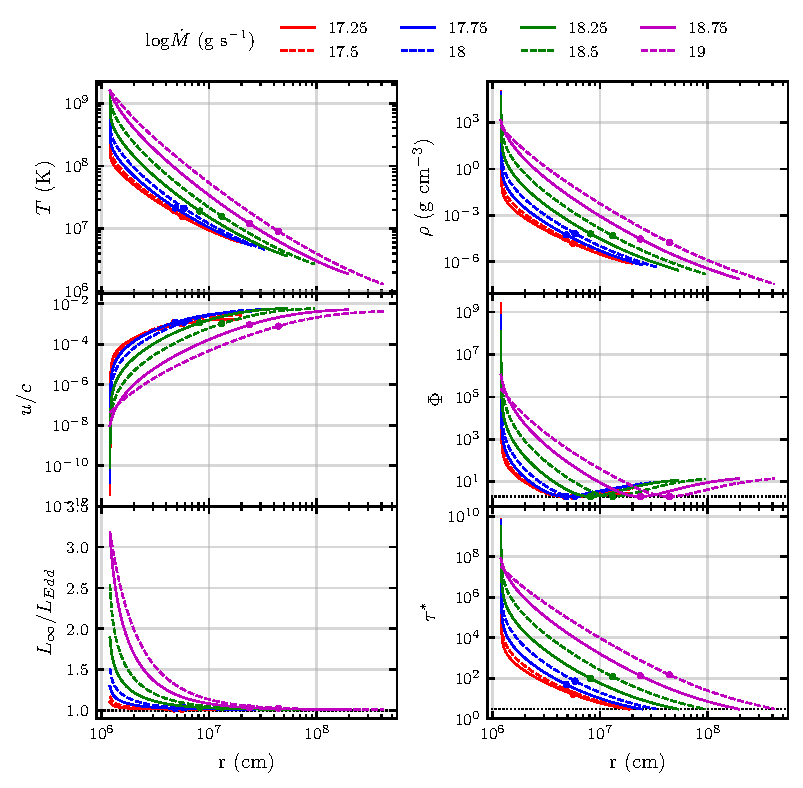
\includegraphics[width=\textwidth]{figures/wind_profiles.pdf}
    \caption[Wind radial profiles]{Wind profiles for different $\Mdot$, from the base $r_b$ to the photosphere $r\ph$. From left to right, up to down : temperature $T$, density $\rho$, velocity $u/c$, velocity parameter $\Phi$, luminosity $L/\Ledd$, optical depth parameter $\tau^*$. The dots indicate the location of the critical point.}
    \label{fig:wind_profiles}
\end{figure}

Since the inner part of the wind is geometrically thin, it is useful to plot certain quantities as a function of density in order to analyze it more clearly. First, as we discussed in the introduction, while the flux seen at infinity can be strongly super-Eddington at the base, the local flux can be sub-critical, which explains the slow rise of the wind. This can clearly be seen in Fig.~\ref{fig:wind_L_Lcrit}. Only the highest $\Mdot$ models start off nearly critical at the base, which is consistent with their higher starting velocities. Past $r_c$ and at $r\ph$, the luminosities are less than 1\% off from $\Lcr$.

\begin{figure}[htb!]
    \centering
    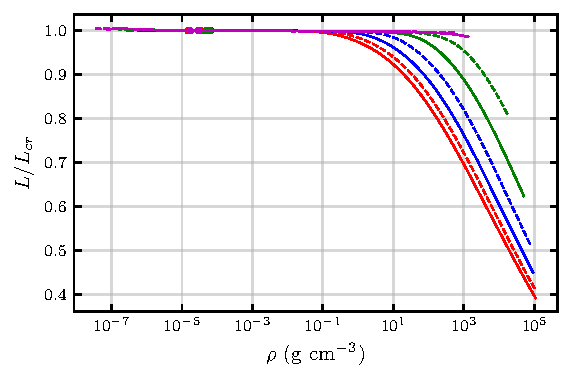
\includegraphics[width=0.7\textwidth]{figures/wind_L_Lcrit.pdf}
    \caption[Wind local to critical luminosity ratios]{Ratios of local luminosity to critical luminosity as a function of density in the wind models. The colors refer to the same legend as Fig.~\ref{fig:wind_profiles}.}
    \label{fig:wind_L_Lcrit}
\end{figure}

Figure \ref{fig:wind_rho_T} shows the temperature as a function of density. As was noted by \citet{Paczynski1986b}, the extended regions of the winds are completely radiation pressure dominated, and they start to transition to a gas pressure dominated regime near the surface as the density increases. The highest $\Mdot$ models however do not transition and remain in the radiation pressure dominated regime. As these authors pointed out, this means that the specific entropy the gas, which sharply drops when going to the gas pressure dominated regime, stays at a high level for the high $\Mdot$ models. Too high, in fact, for any nuclear reaction network to produce enough energy to match to these wind models. Looking at Fig.~\ref{fig:wind_rho_T}, it is clear that the transition to the gas pressure dominated regime simply occurs at a higher density than the other models. Based on this and the discussion on $L
_b^\infty$ in the previous section, it seems that a simple solution to these high $\Mdot$ problems would be to change the inner boundary condition (Eq.~\ref{eq:wind_innerBC}) such that the wind base be defined as having a larger column depth than $10^8$ g cm$^{-2}$. We tried this with $10^9$ g cm$^{-2}$, and realized that non-acceptable wind models still existed, but started at slightly larger values of $\Mdot$. But for this small gain of a larger number of acceptable wind models, the assumption of a pure helium composition becomes less accurate. Indeed, past $y\sim 10
^8$ g cm$^{-2}$, we start to approach nuclear burning regions, where elements such as carbon are expected to be present with significant abundances.  In the end, we decided to keep the original boundary condition, and simply declare our models with $\Mdot\gtrsim 10^{18.5}$ g s$^{-1}$ to be physically non-acceptable\footnote{Note that \citet{Paczynski1986b} rejected models with $\Mdot\geq 10^{19}$ g s$^{-1}$ for the same reasons. They had more acceptable models (larger $\Mdot$ range) because they matched to a higher temperature at the base.}. 

Finally, it appears from Fig.~\ref{fig:wind_rho_T} that degenerate electron corrections are not important for our wind models, even near the base. If we matched to a higher column depth as discussed in the previous paragraph, perhaps they would. So, overall, our wind models agree very well with those of \citet{Paczynski1986b}, which validates our different numerical method and boundary conditions.

%models differ very little from those of \citet{Paczynski1986b}, and we have essentially reproduced their results.

\begin{figure}[htb!]
    \centering
    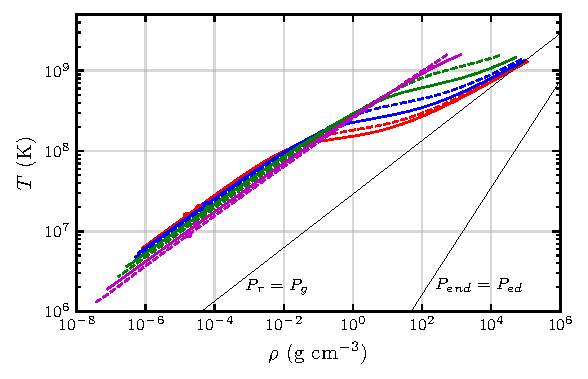
\includegraphics[width=0.7\textwidth]{figures/wind_rho_T.pdf}
    \caption[Wind temperature-density profiles]{Temperature-density profiles in the wind models. The colors refer to the same legend as Fig.~\ref{fig:wind_profiles}. The black lines separate the space in three different pressure regimes. From left to right, pressure is dominated by radiation pressure ($P_r=aT^4/3$), non-degenerate gas pressure ($P_g$), and degenerate gas pressure ($P_\text{ed}$).}
    \label{fig:wind_rho_T}
\end{figure}

\section{Photospheric radii and spectral shifts}\label{sec:wind_photospheres_spectralshifts}
In Chapter \ref{chapter1}, we discussed a recent paper by \citet{Strohmayer2019} which found clear emission and absorption lines in four PRE bursts observed with {\Nicer}. The lines from the stronger bursts were systematically blueshifted relative to the ones from the weaker bursts, which the authors argued could be caused by a combination of gravitational redshift and wind velocity blueshift. Our models can be used to discuss this claim.

First, let us note that our wind models cannot reproduce the inferred photospheric radii of 72 to 103 km found by \citet{Strohmayer2019} -- all of our models have $r\ph>100$ km. This suggests that the PRE phases of these bursts were not caused by a wind, but rather by a series of expanded envelopes (Chapter \ref{chapter4}), in which case there is no blueshift. However, a caveat here is that these radii are derived from blackbody fits. It is known (e.g. \citet{Galloway2017}) that the blackbody temperature of these fits is subject to a color correction factor $f_c\equiv T_\text{BB}/T_\text{eff}$ that can reach values as high as 2, which would make the color-corrected photospheric radius four times larger. The uncertainty around $f_c$, especially in the PRE case, makes it difficult to accurately determine $r\ph$ from observations.

To make sure that our 100 km limit is not a consequence of the neutron star parameters, we computed other wind models with different $M$ and $R$. In Fig.~\ref{fig:spot_check_rphot}, we show the range of photospheric radii in these models as a function of the base luminosity. We see that the minimum value of $r\ph$ depends mostly on $M$, and that even for very light neutron stars, winds have photospheres of over 100 km.

\begin{figure}
    \centering
    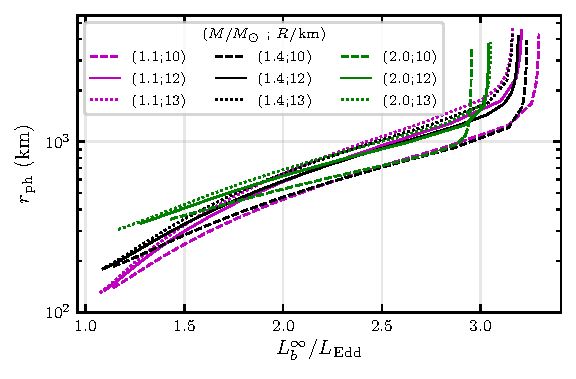
\includegraphics{figures/spot_check_rphot.pdf}
    \caption[Photospheres of winds in different neutron stars]{Photospheric radii for different neutron star masses and radii, as a function of the base luminosity seen by observers at infinity. The solid black line corresponds to the models used throughout this thesis.}
    \label{fig:spot_check_rphot}
\end{figure}

\begingroup
\allowdisplaybreaks
We may still investigate the behavior of spectral shifts, as a function of $r$ for fixed $\Mdot$, and vice-versa. Redshift comes from relativistic curvature,
\begin{equation}
    1+\frac{\Delta\lambda_\text{red}}{\lambda_0}=\left(1-\frac{r_s}{r_0}\right)^{-1/2}=\frac{1}{\zeta}\,,
\end{equation}
\endgroup
where $r_0$ is the emission radius and $\lambda_0$ is the emission wavelength, while blueshift comes from the special relativistic Doppler effect,
\begin{equation}
    1+\frac{\Delta\lambda_\text{blue}}{\lambda_0}=\sqrt{\frac{1-u_0/c}{1+u_0/c}}\,,
\end{equation}
where $u_0$ is the gas velocity at $r_0$. In the top panel of Fig.~\ref{fig:wind_spectral_shifts}, we see that redshift dominates everywhere before the critical point, where it can reach values of several percents. After the critical point and approaching the photosphere, redshift and blueshift become comparable to the point where the total spectral shift is close to zero. We can see from the bottom panel of Fig.~\ref{fig:wind_spectral_shifts} that for every wind model, the total shift at the photosphere is of less than 1\%. This is not enough to produce the relative line shift of 1.046 in \citet{Strohmayer2019},. It is interesting to note the changing sign of $\Delta\lambda$ at high $\Mdot$, as both velocities and photospheric radii increase, although being able observing such small shifts is unlikely.

We must also note that there is no guarantee that the emission radius of spectral lines is at the Helium photosphere. Heavier elements that are thought to be ejected have more complex interactions with radiation, and absorption/emission lines themselves are not a continuum effect, which is how radiation is treated in our model. Our wind models can describe the relative importances of redshift and blueshift, but true predictions on spectral lines will require a more sophisticated treatment of radiative transfer.

\begin{figure}[H]
    \centering
    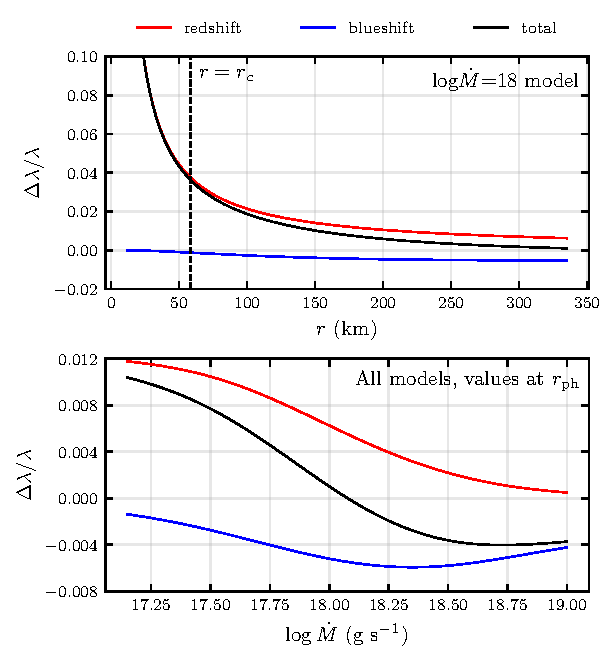
\includegraphics{figures/wind_lineshift.pdf}
    \caption[Wind spectral shifts]{Wind spectral shifts, as a function of radii for the $\log\Mdot=18$ model (\textit{top}), and as a function of $\Mdot$ at the photosphere (\textit{bottom}).}
    \label{fig:wind_spectral_shifts}
\end{figure}


% more on shifts: (color corrected means higher photosphere), for smaller photospheres can get 1% shifts, but need better models


\biblio
\end{document}
